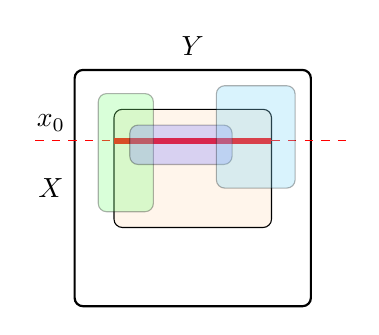
\begin{tikzpicture}
    \draw[thick, rounded corners = 3pt] (0, 0) rectangle (3, -3);
    \draw[fill = orange!8, rounded corners = 3pt] (0.5, -0.5) rectangle (2.5, -2);
    \node at (-0.3, -1.5) {$X$};
    \node at (1.5, 0.3) {$Y$};

    \node[above] at (-0.3, -0.9) {$x_0$};
    \draw[red, dashed] (-0.5, -0.9) -- (0.5, -0.9);
    \draw[line width = 2pt, red] (0.5, -0.9) -- (2.5, -0.9);
    \draw[red, dashed] (2.5, -0.9) -- (3.5, -0.9);

    \pause
    \only<2->{
        \draw[fill = green!50, rounded corners = 3pt, opacity = 0.3] (0.3, -0.3) rectangle (1, -1.8);
        \draw[fill = blue!50, rounded corners = 3pt, opacity = 0.3] (0.7, -0.7) rectangle (2, -1.2);
        \draw[fill = cyan!50, rounded corners = 3pt, opacity = 0.3] (1.8, -1.5) rectangle (2.8, -0.2);
    }

    \onslide<1->
\end{tikzpicture}
